\section{Aging walks}\label{sec:aging}

In this section the walk remembers its age. After its first step it switches
direction at step $k\ge2$ with probability $c/k$, independently of the past,
where $0<c<2$. So the walk switches less and less often, and the expected
number of switches in $N$ steps is $c(H_N-1)$, which is about $c\log N$. With
a fair first step, $A_N/N$ converges in law to
$\mathrm{Beta}(c,c)$~\cite[Example~1.1 and Theorem~1.4]{ds2007} (their chain
is this walk for $c\le1$), \cite[Theorem~1]{ev2018}, and the limit is uniform
exactly when $c=1$~\cite[Remark~2]{ev2018}. At finite $N$ the first step
matters. We first fix it, then pass to $d$ states, and then return to the
fair first step.

We write $\Prob_+$ for the law given $X_1=+1$, as in
Section~\ref{sec:heavy}, and $X_N$ for the last step. A path is a sequence
$x\in\{\pm1\}^N$, and it switches at time $t\ge2$ if $x_t\ne x_{t-1}$. Step
$k\ge2$ contributes the factor $c/k$ to the probability of a path if the path
switches there, and $1-c/k$ otherwise. So relative to no switch, a switch at
time $t$ multiplies the probability of a path by the odds
\[
 \omega_t=\frac{c/t}{1-c/t}=\frac{c}{t-c}\qquad(t\ge2),
\]
and
\begin{equation}\label{eq:aging-path}
 \Prob_+(X=x)=\prod_{k=2}^N\Bigl(1-\frac ck\Bigr)\prod_{t:\,x_t\ne x_{t-1}}\omega_t
 \qquad(x_1=+1).
\end{equation}
Each $\omega_t$ is positive and continuous on $(0,2)$, increases strictly in
$c$, and tends to $0$ as $c\downarrow0$.

\subsection{A fixed first step}

\begin{proposition}[two states, fixed first step]\label{prop:aging-two}\label{rem:aging}
Let $N\ge2$ and let the first step be $+1$.
\begin{enumerate}[(a)]
\item At $c=1$, for $1\le s\le N$,
\[
 \Prob_+(A_N=s,\,X_N=+1)=\frac{s-1}{N(N-1)},\qquad
 \Prob_+(A_N=s,\,X_N=-1)=\frac{N-s}{N(N-1)}.
\]
So $A_N$ is uniform on $\{1,\dots,N\}$.
\item For $1\le s\le N-1$ the ratio $\Prob_+(A_N=s)/\Prob_+(A_N=N)$ increases
strictly in $c\in(0,2)$, and it equals $1$ exactly at $c=1$.
\end{enumerate}
\end{proposition}

In words, with a fixed first step every bin from $1$ to $N-1$ ties with the
end bin $N$ at $c=1$, for every $N$. For $c<1$ the end bin is the most likely
bin, and for $c>1$ it is the least likely of the bins $1,\dots,N$ (bin $0$
has probability $0$). So the fixed-start crossing is exactly $c=1$, and it
does not depend on $N$ or on the bin.

\begin{proof}
(a) We use induction on $N$. Put $u^\pm_N(s)=\Prob_+(A_N=s,\,X_N=\pm1)$, which
is $0$ unless $1\le s\le N$. For $N=2$ the second step is $+1$ or $-1$ with
probability $\frac12$ each, so $u^+_2(2)=u^-_2(1)=\frac12$ and
$u^+_2(1)=u^-_2(2)=0$, as claimed. At $c=1$ step $N+1$ switches with
probability $1/(N+1)$. Conditioning on $X_N$ gives, for every $s$,
\[
 (N+1)\,u^+_{N+1}(s+1)=N\,u^+_N(s)+u^-_N(s),\qquad
 (N+1)\,u^-_{N+1}(s)=u^+_N(s)+N\,u^-_N(s).
\]
Suppose the claim holds for $N$, and let $1\le s\le N$. Then
$N(s-1)+(N-s)=s(N-1)$ gives $u^+_{N+1}(s+1)=\frac{s}{(N+1)N}$, and
$(s-1)+N(N-s)=(N-1)(N+1-s)$ gives $u^-_{N+1}(s)=\frac{N+1-s}{(N+1)N}$. The
two remaining values are $u^+_{N+1}(1)=0$ and $u^-_{N+1}(N+1)=0$, since
$u^\pm_N(0)=u^\pm_N(N+1)=0$. This is the claim for $N+1$. Summing over $X_N$
gives $\Prob_+(A_N=s)=\frac{(s-1)+(N-s)}{N(N-1)}=\frac1N$.

(b) We write the ratio as a sum over paths. Only the path with every step
$+1$ has $A_N=N$, and it never switches. So $\Prob_+(A_N=N)$ is the first
product in~\eqref{eq:aging-path}, and dividing by it leaves
\begin{equation}\label{eq:aging-ratio}
 \frac{\Prob_+(A_N=s)}{\Prob_+(A_N=N)}
 =\sum_{x}\ \prod_{t:\,x_t\ne x_{t-1}}\omega_t ,
\end{equation}
where the sum is over the paths $x$ with $x_1=+1$ and $s$ steps equal to
$+1$. For example, for $N=3$ and $s=2$ the paths are $(+,+,-)$ and $(+,-,+)$,
and the ratio is $\omega_3+\omega_2\omega_3$. For $1\le s\le N-1$ there is
such a path, and each of them switches at least once. So the right side is a
sum of products of the $\omega_t$ with at least one factor each. Each
$\omega_t$ is positive and increases strictly in $c$, so the sum does too. By
(a) it equals $1$ at $c=1$.
\end{proof}

After a shift of one step, part (a) is the exercise
in~\cite[footnote~1 on p.~6]{evw2020}. That footnote also says that the fact
can be related to P\'olya urns (the authors credit M.~Bal\'azs) and that a
more general connection of their model with P\'olya urns will appear in a
later paper. So the uniform law for two states is not new. What we add for
two states is the joint law with the last step and part (b). The argument for
(b) is the one in
Proposition~\ref{prop:mlr}. Both parts of
Proposition~\ref{prop:aging-two} are also proved in Lean
(Section~\ref{sec:verify}).

\subsection{\texorpdfstring{$d$}{d} states}

The same thing happens for a chain on $d$ states that leaves its current
state for each other state at the same aging rate. For such chains Dietz and
Sethuraman~\cite[Theorem~1.4]{ds2007} proved that the fractions of time
converge in law to the Dirichlet law with every parameter $\theta$, which is
uniform on the simplex exactly at $\theta=1$ (see also~\cite{bc2018}). Their
chain moves to each other state with probability $\theta/n$ at time $n$ once
$n>\lceil(d-1)\theta\rceil$, and it does not move before that. Ours, defined
below for $\theta<d/(d-1)$, moves to each other state with probability
$\theta/(k+d-2)$ at every step $k\ge2$. If $\theta\le1$ then
$\lceil(d-1)\theta\rceil\le d-1$, so our step $k$ has the transition
probabilities of their time $k+d-2$ for every $k\ge2$, and the two chains
differ by a shift of $d-2$ steps. If $\theta>1$ the ceiling is $d$. Then
their chain stays at time $d$, where ours takes its second step, and the
later steps agree. One step does not change the limit.
Part (a) of the theorem below is an exact form of their limit at finite $N$.
Fix $d\ge2$ and $\theta$
with $0<\theta<d/(d-1)$. The chain $X_1,X_2,\dots$ on $\{1,\dots,d\}$ starts at
$X_1=1$. At step $k\ge2$ it moves to each of the other $d-1$ states with
probability $\theta/(k+d-2)$, and it stays with probability
$1-(d-1)\theta/(k+d-2)$. The condition on $\theta$ says that the probability
of staying is positive at every step $k\ge2$. Let
$L_N=(L_N(1),\dots,L_N(d))$ be the vector of visit counts, namely
$L_N(i)=\#\{k\le N:X_k=i\}$. Its values are the compositions
$n=(n_1,\dots,n_d)$ of $N$ into $d$ nonnegative parts with $n_1\ge1$. There
are $\binom{N+d-2}{d-1}$ of them (subtract one from $n_1$). We call them
bins. The corner $Ne_1$, where $e_i$ is the $i$-th unit vector, is the bin of
the chain that never moves.

\begin{theorem}[$d$ states]\label{thm:aging-d}
Let $d\ge2$, $0<\theta<d/(d-1)$ and $N\ge2$.
\begin{enumerate}[(a)]
\item At $\theta=1$, for every bin $n$ and every state $j$,
\begin{equation}\label{eq:aging-d}
 \Prob(L_N=n,\,X_N=j)=\frac{n_j-\mathbf 1\{j=1\}}{(N-1)\binom{N+d-2}{d-1}} .
\end{equation}
So $L_N$ is uniform on the $\binom{N+d-2}{d-1}$ bins, the corner included.
\item For every bin $n\ne Ne_1$ the ratio $\Prob(L_N=n)/\Prob(L_N=Ne_1)$
increases strictly in $\theta$, and it equals $1$ exactly at $\theta=1$.
\end{enumerate}
\end{theorem}

In words, at $\theta=1$ all bins are equally likely, and given the counts the
last state is distributed as the state at a uniformly chosen one of the steps
$2,\dots,N$ (the forced first visit to state $1$ is left out). Every other bin
ties with the corner exactly at $\theta=1$, for every $N\ge2$ and every $d$.
Below $\theta=1$ the corner is the most likely bin, and above it the corner
is the least likely.

\paragraph{Idea of the proof.}
For (a) we check~\eqref{eq:aging-d} by induction on $N$. At $\theta=1$ step
$N$ stays with weight $N-1$ and moves to each other state with weight $1$. We
read the weight $N-1$ as $(N-2)+1$. So the chain copies its last state with
weight $N-2$, and it picks each of the $d$ states with weight $1$. By the
induction hypothesis the last state is like the state at a uniformly chosen
one of the steps $2,\dots,N-1$. So given the counts $m$ after $N-1$ steps, the
new state is $j$ with weight $(m_j-\mathbf 1\{j=1\})+1$. This is the rule of
P\'olya's urn, and it keeps the counts uniform. Part (b) is the path-weight
argument of Proposition~\ref{prop:aging-two}(b).

\begin{proof}
(a) We use induction on $N$. Write $P_N(n,j)=\Prob(L_N=n,\,X_N=j)$ and
$\delta_j=\mathbf 1\{j=1\}$. Let $N=2$. At $\theta=1$ the second step goes to each
of the $d$ states with probability $1/d$ (the probability of staying is
$1-(d-1)/d$). So $P_2(2e_1,1)=\frac1d$ and $P_2(e_1+e_j,j)=\frac1d$ for
$j\ne1$, and $P_2$ vanishes otherwise. Since $\binom d{d-1}=d$, the right
side of~\eqref{eq:aging-d} is $(n_j-\delta_j)/d$. This is $\frac1d$ in these $d$
cases. In every other case $n_j=\delta_j$, and it is $0$.

Now let $N\ge3$ and suppose that~\eqref{eq:aging-d} holds for $N-1$. Fix a bin
$n$ and a state $j$. If $n_j=\delta_j$, then the right side of~\eqref{eq:aging-d}
is $0$. The left side is $0$ too. Indeed, if $j\ne1$ then state $j$ is never
visited, and if $j=1$ then state $1$ is visited only at the first step, so
$X_N\ne j$ in both cases. Otherwise $m=n-e_j$ is a composition of $N-1$ with
$m_1\ge1$. At $\theta=1$ step $N$ moves to each other state with probability
$1/(N+d-2)$ and stays with probability $(N-1)/(N+d-2)$. Conditioning on
$X_{N-1}$ gives
\[
 P_N(n,j)=\frac{(N-1)\,P_{N-1}(m,j)+\sum_{i\ne j}P_{N-1}(m,i)}{N+d-2}
 =\frac{(N-2)\,P_{N-1}(m,j)+\sum_{i}P_{N-1}(m,i)}{N+d-2} .
\]
By the induction hypothesis and $\sum_i(m_i-\delta_i)=N-2$, the numerator is
\[
 \frac{(N-2)(m_j-\delta_j)+(N-2)}{(N-2)\binom{N+d-3}{d-1}}
 =\frac{n_j-\delta_j}{\binom{N+d-3}{d-1}} .
\]
Since $\binom{N+d-2}{d-1}=\binom{N+d-3}{d-1}\frac{N+d-2}{N-1}$, this
gives~\eqref{eq:aging-d} for $N$. Summing~\eqref{eq:aging-d} over $j$ and
using $\sum_j(n_j-\delta_j)=N-1$ gives $\Prob(L_N=n)=1/\binom{N+d-2}{d-1}$.

(b) A path $x\in\{1,\dots,d\}^N$ with $x_1=1$ has probability
$\prod_{k=2}^N\bigl(1-\frac{(d-1)\theta}{k+d-2}\bigr)$ times the product of
the odds
\[
 \omega^{(d)}_t=\frac{\theta/(t+d-2)}{1-(d-1)\theta/(t+d-2)}
 =\frac{\theta}{t+d-2-(d-1)\theta}
\]
over the times $t\ge2$ with $x_t\ne x_{t-1}$. The denominator is positive and
decreases in $\theta$, so each $\omega^{(d)}_t$ increases strictly in
$\theta$. Only the constant path has counts $Ne_1$. So
$\Prob(L_N=n)/\Prob(L_N=Ne_1)$ is the sum of the products of the odds over
the paths with counts $n$. For a bin $n\ne Ne_1$ there is such a path, and
each of them moves at least once. Hence the ratio increases strictly in
$\theta$, and by (a) it equals $1$ at $\theta=1$.
\end{proof}

\begin{remark}\label{rem:aging-d}
For $d=2$ the chain switches at step $k$ with probability $\theta/k$, so
Theorem~\ref{thm:aging-d} with $\theta=c$ is
Proposition~\ref{prop:aging-two}, and~\eqref{eq:aging-d} reads
$(s-1)/(N(N-1))$ for $j=1$ and $n=(s,N-s)$.

Take P\'olya's urn with $d$ colors, started with one ball of each color. At
each draw we take a ball uniformly at random and return it with one more
ball of its color. A sequence of $N-1$ draws with counts $m$ has probability
$(d-1)!\prod_im_i!/(N+d-2)!$. So the counts are uniform on the compositions
of $N-1$ into $d$ parts, and given the counts $m$ the last draw has color $j$
with probability $m_j/(N-1)$. Hence~\eqref{eq:aging-d} says that, for each
fixed $N$, the pair $(L_N-e_1,X_N)$ has the law of the counts and the last
color after $N-1$ draws. The two processes are different, though. The
chain is a Markov chain, and the draws are exchangeable. For $d=2$ and $N=4$
the path $1,1,2,2$ has probability $\frac18$ for the chain, and the draws
$1,2,2$ have probability $\frac1{12}$. Also, at $\theta=1$ the chain moves at
step $k$ with probability $(d-1)/(k+d-2)$, independently over $k$. This is
the probability that customer $k$ opens a new table in the Chinese restaurant
process with parameter $d-1$. So the expected number of moves in $N$ steps at
the tie is $\sum_{k=2}^N\frac{d-1}{k+d-2}=(d-1)\log N+O(1)$, which is the
first-order scale of the vertex crossing in Paper~B~\cite{paperB}.

We checked~\eqref{eq:aging-d} and the strict ordering in (b) in exact
rational arithmetic for $d=2,3,4$ and $2\le N\le8$
(\texttt{verify\_aging.py}).
\end{remark}

The urn is not special to $\theta=1$. It appears for every weight once the
aging rate is adjusted a little. The chain below either redraws its state or
repeats it. This is the mechanism of the conservative random walk of
Engl\"ander and Volkov~\cite{ev2022}, who redraw a direction in $\mathbb Z^d$
with probability $p_n$ and study recurrence and scaling limits. We do not
claim the urn law below as new. The footnote quoted above announces a general
connection with P\'olya urns, and two chapters of the book~\cite{ev2024} concern
urn models. We have not seen them. What we use it for is the explicit joint law on
$d$ states and the tie. Fix $d\ge2$ and $\theta>0$, and let
$Y_1,Y_2,\dots$ be the following chain on $\{1,\dots,d\}$. At step $t\ge1$,
with probability
\[
 \varphi_t=\frac{d\theta}{d\theta+t-1}
\]
the state $Y_t$ is drawn afresh, uniformly from the $d$ states, and otherwise
$Y_t=Y_{t-1}$ (so $Y_1$ is uniform, since $\varphi_1=1$). In other words, at
step $t\ge2$ the chain moves to each other state with probability
$\theta/(d\theta+t-1)$. Let $M_T$ be the vector of visit counts of
$Y_1,\dots,Y_T$. At $\theta=1$ this is the chain of
Theorem~\ref{thm:aging-d} without its first step, namely $Y_t=X_{t+1}$ and
$M_T=L_{T+1}-e_1$. We write $x^{(m)}=x(x+1)\cdots(x+m-1)$.

\begin{proposition}[fresh or repeat]\label{prop:aging-urn}
For every $T\ge1$, every composition $m$ of $T$ into $d$ nonnegative parts and
every state $j$,
\begin{equation}\label{eq:aging-urn}
 \Prob(M_T=m,\,Y_T=j)=\frac{m_j}{T}\,D_T(m),\qquad
 D_T(m)=\frac{T!}{(d\theta)^{(T)}}\prod_{i=1}^d\frac{\theta^{(m_i)}}{m_i!} .
\end{equation}
So $M_T$ has the law $D_T$ of the counts in P\'olya's urn with $d$ colors and
initial weight $\theta$ on each color. For $d=2$ and even $T$,
\begin{equation}\label{eq:aging-urn-ratio}
 \frac{\Prob(M_T=(T/2,T/2))}{\Prob(M_T=(T,0))}
 =\binom{T}{T/2}\prod_{i=0}^{T/2-1}\frac{\theta+i}{\theta+T/2+i},
\end{equation}
which increases strictly in $\theta$ and equals $1$ exactly at $\theta=1$.
\end{proposition}

In words, the chain repeats its last state where the urn repeats a uniformly
chosen earlier draw, and at each fixed time this makes no difference to the
counts or to the last state. For two states the center and the end tie at
$\theta=1$ for every $T$, with ends ahead below it and the center ahead above
it, and now the whole law is explicit on both sides of the tie
(Figure~\ref{fig:aging}).

\begin{figure}[t]
\centering
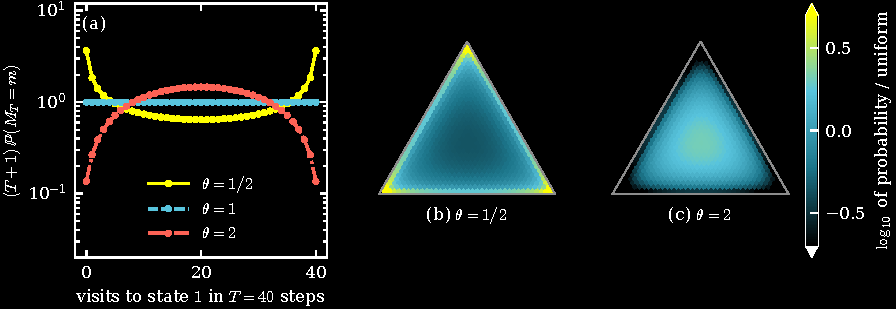
\includegraphics[width=\textwidth]{figures/aging}
\caption{The exact law~\eqref{eq:aging-urn} of the counts of the chain that
draws afresh or repeats. (a) Two states and $T=40$, as a multiple of the
uniform law. The law is flat at $\theta=1$, the ends are the most likely bins
for $\theta=\frac12$, and the center is for $\theta=2$. (b), (c) Three states
and $T=36$ on the simplex of visit fractions. Each cell is one bin, colored by
its probability relative to the uniform law. For $\theta=\frac12$ a corner is
$9.6$ times as likely as under the uniform law and the center $0.43$ times.
For $\theta=2$ the numbers are $0.035$ and $2.1$.}
\label{fig:aging}
\end{figure}

\begin{proof}
We use induction on $T$. For $T=1$ both sides of~\eqref{eq:aging-urn} are
$\frac1d$ when $m=e_j$ and $0$ otherwise. Let $T\ge2$ and suppose
\eqref{eq:aging-urn} holds for $T-1$. If $m_j=0$ both sides vanish. Otherwise
put $m'=m-e_j$. Summing~\eqref{eq:aging-urn} over the last state gives
$\Prob(M_{T-1}=m')=D_{T-1}(m')$. A fresh draw gives $j$ with probability
$\frac1d$ whatever the last state was, and a repeat gives $j$ only when the
last state was $j$ (this is why the induction carries the last state along
with the counts). So
\[
 \Prob(M_T=m,\,Y_T=j)
 =\frac{\varphi_T}{d}\,D_{T-1}(m')+(1-\varphi_T)\,\frac{m_j-1}{T-1}\,D_{T-1}(m')
 =\frac{\theta+m_j-1}{d\theta+T-1}\,D_{T-1}(m') .
\]
On the other hand
$D_T(m)=D_{T-1}(m')\cdot\frac{T}{m_j}\cdot\frac{\theta+m_j-1}{d\theta+T-1}$ by
the definition of $D_T$. This gives~\eqref{eq:aging-urn}. Summing over $j$
gives $\Prob(M_T=m)=D_T(m)$, and the ratio~\eqref{eq:aging-urn-ratio} is
$D_T(T/2,T/2)/D_T(T,0)$ with
$\theta^{(T)}=\theta^{(T/2)}(\theta+T/2)^{(T/2)}$. Each factor
$(\theta+i)/(\theta+T/2+i)$ increases strictly in $\theta$, and at
$\theta=1$ the product is $(T/2)!^2/T!$.
\end{proof}

\begin{remark}\label{rem:aging-feller}
Here is another way to see the law of the counts in
Proposition~\ref{prop:aging-urn} (but not the joint law with the last state).
The fresh draws
cut $Y_1,\dots,Y_T$ into runs, and each run gets a uniform state. The urn can
be run in the same way, as a Chinese restaurant process in which each table
gets a uniform color. There a table is opened with the same probabilities
$\varphi_t$. The lengths of the runs are the spacings between the successes of
independent trials with success probabilities $\varphi_t$, and it is a classical
fact (the Feller coupling, see~\cite{abt2003}) that these spacings have
the same law as the table sizes. We do not know whether this is the relation
to P\'olya urns that the footnote of~\cite{evw2020} has in mind. We
checked~\eqref{eq:aging-urn} in exact arithmetic for four values of $\theta$,
with $T\le7$ for $d=2,3$ and $T\le5$ for $d=4$
(\texttt{verify\_aging\_urn.py}).
\end{remark}

\subsection{A fair first step}

We return to two states and let the first step be fair. Then both ends can be
reached, and $E_N=\Prob(A_N=N)=\frac12\prod_{k=2}^N(1-c/k)$. Changing the sign
of every step preserves the law of the walk and sends $A_N$ to $N-A_N$. So
\begin{equation}\label{eq:aging-fair}
 \Prob(A_N=s)=\tfrac12\bigl(\Prob_+(A_N=s)+\Prob_+(A_N=N-s)\bigr),\qquad
 E_N=\tfrac12\Prob_+(A_N=N),
\end{equation}
since $\Prob_+(A_N=0)=0$.

\begin{proposition}[fair first step]\label{prop:aging-fair}
Let $N\ge2$ and $1\le s\le N-1$, with a fair first step.
\begin{enumerate}[(a)]
\item At $c=1$, $\Prob(A_N=s)=\frac1N$ and $E_N=\frac1{2N}$.
\item The ratio $\Prob(A_N=s)/E_N$ is continuous and strictly increasing in
$c\in(0,2)$. It tends to $0$ as $c\downarrow0$ and equals $2$ at $c=1$. So
there is exactly one $c$ in $(0,2)$ with $\Prob(A_N=s)=E_N$, and it is less
than $1$.
\end{enumerate}
\end{proposition}

For even $N$ we write $c_N$ for the crossing in (b) with $s=h=N/2$, so that
$C_N=E_N$ exactly at $c=c_N$. In words, at $c=1$ every interior bin still has
probability $\frac1N$, and the two ends share the probability $\frac1N$ that
the fixed start gave to one end. So at $c=1$ the center is twice as likely as
an end, and the crossing moves below $1$.

\begin{proof}
(a) This follows from~\eqref{eq:aging-fair} and
Proposition~\ref{prop:aging-two}(a). (b) By~\eqref{eq:aging-fair} the ratio
is the sum of the right sides of~\eqref{eq:aging-ratio} for $s$ and for
$N-s$. Both are finite sums of products of at least one $\omega_t$. So the
ratio is continuous and strictly increasing, and it tends to $0$ as
$c\downarrow0$. By (a) it equals $2$ at $c=1$. Hence it equals $1$ exactly
once, at some $c<1$.
\end{proof}

How far below $1$ is $c_N$? The end is of order $N^{-c}$ and the center is of
order $1/N$, so they meet when $N^{1-c}$ is about $2$.

\begin{proposition}[the fair-start crossing]\label{prop:aging-expansion}
For even $N\to\infty$,
\[
 c_N=1-\frac{\log2}{\log N+\gamma+2-2\log2}+O\bigl((\log N)^{-3}\bigr),
\]
where $\gamma$ is Euler's constant.
\end{proposition}

\paragraph{Idea of the proof.}
The end is explicit, namely
$E_N=\Gamma(N+1-c)/(2\Gamma(2-c)\Gamma(N+1))$, which is
$N^{-c}/(2\Gamma(2-c))$ with relative error $O(1/N)$. For the center we prove
a local limit theorem with a rate, namely $NC_N=d_c+O(N^{-0.4})$ uniformly
for $c$ near $1$, where $d_c=4^{1-c}/\mathrm B(c,c)$ is the density of
$\mathrm{Beta}(c,c)$ at $\frac12$. So
$\log(C_N/E_N)=(c-1)\log N+\Theta(c)+O(N^{-0.4})$ with
$\Theta(c)=\log(2\Gamma(2-c)d_c)$. Here $\Theta(1)=\log2$ and
$\Theta'(1)=\gamma+2-2\log2$, and solving for the zero gives the expansion.
The proof is in Appendix~\ref{app:aging}. The local limit theorem comes from
an averaging identity for $C_N$ and a coupling of the walk with a sign
process driven by a Poisson process of intensity $c\,dt/t$, whose occupation
fraction is exactly $\mathrm{Beta}(c,c)$.

The convergence is slow. The exact crossing at $N=200$ is $c_{200}=0.8925$,
against $0.8932$ from the expansion without its error term. The constant in
the error term is not computed.
